%!TEX root = ../dissertation.tex
\newpage
\thispagestyle{empty}
	
% If you do want an image in the colophon:
%\begin{figure}
  \vspace{10pt}
  \centering
%  \hspace*{-32pt}
  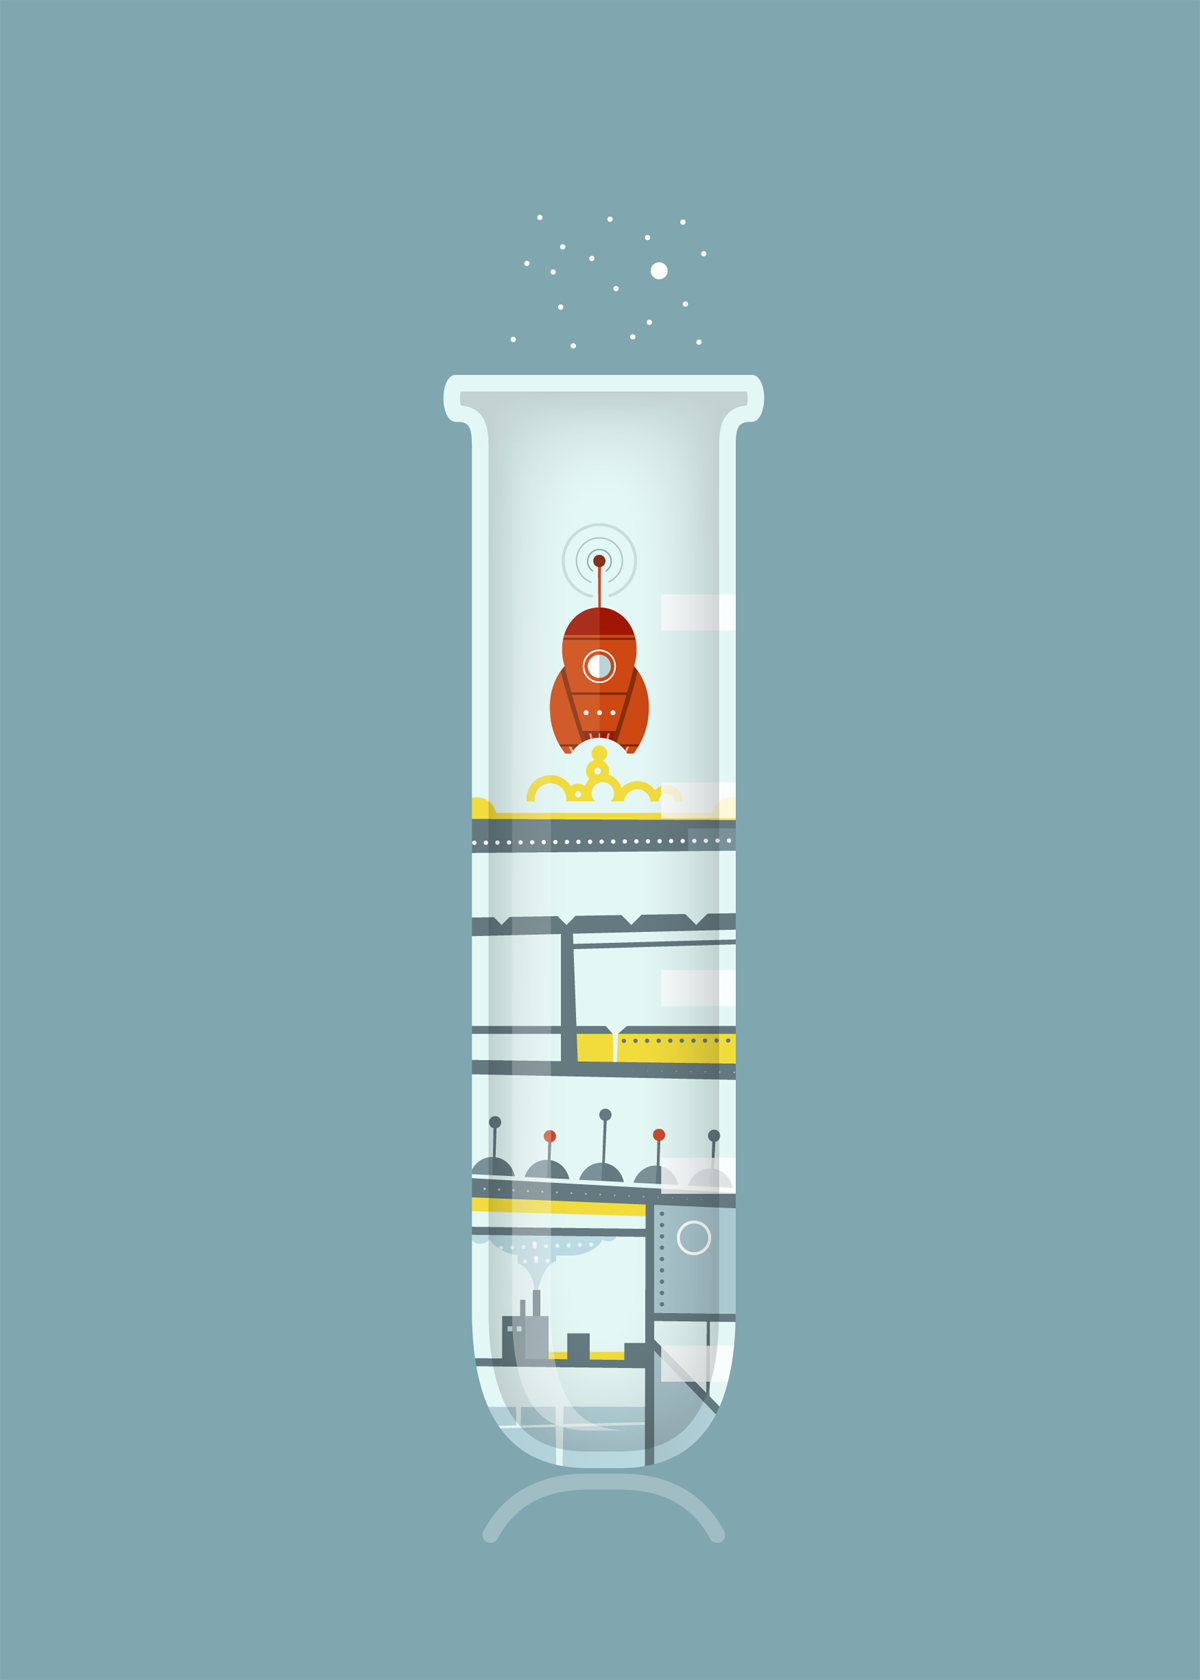
\includegraphics[width=0.42\textwidth]{endmatter/colophon.png}
%\end{figure}

% If you don't want an image in the colophon:
% \vspace*{200pt}
\vspace{20pt}

\begin{center}
\parbox{220pt}{\small \lettrine[lines=3,slope=-2pt,nindent=-4pt]{\textcolor{SchoolColor}{T}}{his thesis was typeset} 
using \LaTeX, originally developed by Leslie Lamport and based on Donald Knuth's \TeX. 
The body text is set in 11~point Minion Pro, designed by Robert Slimbach in 1990 inspired by late Renaissance-era type and issued by Adobe in 2000.
The headlines and captions are set in variations of Myriad Pro, a humanist sans-serif typeface designed by Robert Slimbach and Carol Twombly in 1990 and issued by Adobe in 2000.
The above illustration %, \textit{Science Experiment 02}, 
was created by \href{http://www.studiobenben.com/27771/428167/projects/science-experiments}{Ben Schlitter} 
and released under \href{http://creativecommons.org/licenses/by-nc-nd/4.0/}{\textsc{cc by-nc-nd 4.0}}. 
A template that can be used to format a PhD dissertation with this look \textit{\&} feel has been released under the permissive \href{http://www.gnu.org/licenses/agpl-3.0.html}{\textsc{agpl}} license, and can be found online at \href{https://github.com/aminmkhan/Dissertate}{github.com/aminmkhan/Dissertate}
or from its lead author, \href{https://github.com/suchow}{Jordan Suchow}, at \href{mailto:suchow@post.harvard.edu}{suchow@post.harvard.edu}.}
\end{center}
